\head{Февраль}{Листок 6. Метод математической индукции.}

\section*{Страдания двоечника Васи.}

В тексте общего характера, как известно читателям книжек про Шерлока Холмса, слово ''индукция'' означает \textit{''рассуждение от частного к общему''} - в противовес дедукции, \textit{''рассуждению от общего к частному''}. Примеры бытовой индукции часто можно услышать в разговорах: \textit{''У меня было трое знакомых по имени Вася и все они оказались дураками. Ясное дело, все Васи такие''}. Некорректность этого вывода очевидна даже тем, кто никогда не слыхал ни про Жуковского, ни про Тредиаковского. Более корректный вывод про Васю можно найти в анналах средней школы села Липовое.\footnote{Печальная история двоечника Васи была любезно предоставлена нам А.С.Головановым (ГУАСом)}

Жил-был в селе Липовое двоечник Вася. Получал он двойки по всем предметам и в большом количестве. И что бы с ним учителя не делали, от двоек этих никак не мог он избавиться. И так он достал
всех учителей, что решили они навести порядок среди двоек и созвали однажды педсовет, который, как говорят, единогласно принял два решения:
\begin{enumerate}
\item Каждый понедельник ученик Вася Пупкин должен получать двойку.
\item Если учитель видит в журнале, что вчера Вася получил двойку, сегодня ему тоже нужно поставить двойку - так ему, двоечнику!
\end{enumerate}

Интересно, что произойдёт в субботу? Согласно 1. в понедельник Васе двойка обеспечена. Тогда (см. 2.) бедный мальчик получит двойку и во вторник. А раз во вторник, то и в среду. Потом в четверг. Потом в пятницу. Значит, и в субботу!

Представляется интуитивно очевидным, что если бы школу не закрывали в воскресенья и каникулы, череда Васиных двоек продлилась бы бесконечно.

Мы вплотную подошли к осознанию \textit{принципа математической индукции}. В истории про Васю речь идёт о конечном числе шагов. В принципе математической индукции мы оперируем бесконечным
числом шагов. Можно попробовать сформулировать его так:

\fbox{\begin{minipage}{0.95\textwidth}
    Если число 1 обладает некоторым свойством, и вместе с каждым натуральным числом $n$ этим свойством обладает следующее за ним число $n+1$, то этим свойством обладают вообще все натуральные числа.
\end{minipage}} 

\begin{samp}
Если число 1 - хорошее, и из того, что число $n$ - хорошее следует, что число $n+1$ - хорошее, получаем, что тогда все натуральные числа хорошие. \smiley
\end{samp}

\begin{center}
    \textbf{А теперь просто задача.}
\end{center}

\begin{thm} \label{6.0 thm1}
Из квадрата $16 \cdot 16$ произвольно вырезали одну клетку. Докажите, что полученную фигуру можно разрезать на ''уголки'' из
трёх клеток.
\end{thm}

{\setlength{\intextsep}{2pt}
\begin{figure}[h]
\begin{minipage}{0.72\linewidth}\setlength{\parindent}{1.5em}
\textbf{\textit{Решение.}} Попытаемся сначала решить более простую аналогичную задачу. 
Во-первых, уменьшим размеры квадрата (например, до $4 \cdot 4$ или $2 \cdot 2$), а, во-вторых, временно зафиксируем вырезанную клетку в углу квадрата. Ну, с квадратом $2 \cdot 2$, вообще всё просто, - какую бы клетку мы не вырезали, оставшиеся три клетки образуют требуемый ''уголок'' (рис. 1а). А что же делать в квадрате $4 \cdot 4$? Разрежем его на четыре квадратика $2 \cdot 2$. 
\end{minipage}
\hfill
\begin{minipage}{0.25\linewidth}
    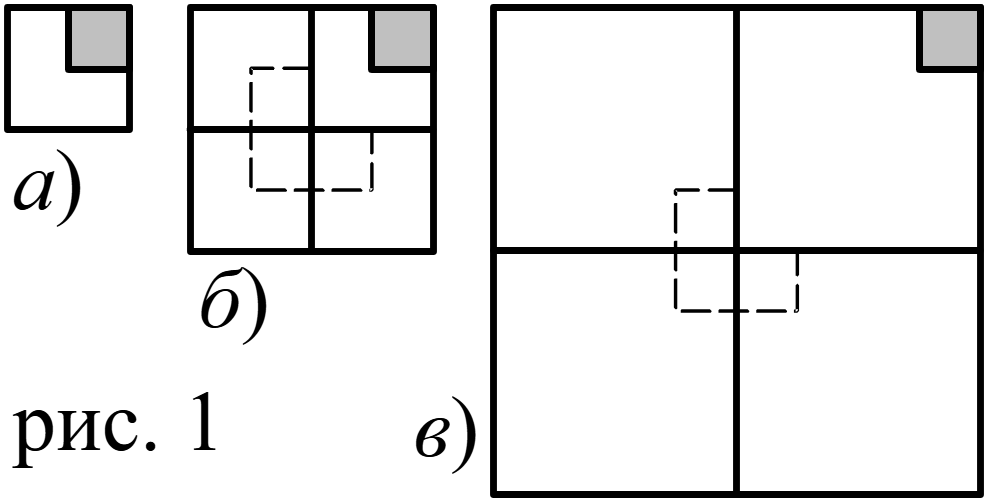
\includegraphics[scale=0.8]{img/kvadrat1.png}
\end{minipage}
\end{figure}}

С тем, у которого имеется вырезанная клетка, всё ясно. Если далее попытаться разрезать оставшийся ''большой уголок'' на маленькие, то оказывается, что это можно сделать единственным способом (вспомните известную задачу на разрезание уголка из трёх квадратов), причём один из получившихся уголков будет принадлежать всем трем квадратикам $2 \cdot 2$ (рис. 1б), вырезая из каждого именно
угловую клетку. 
Попробуем теперь разрезать на уголки квадрат $8 \cdot 8$ с вырезанным уголком. Делим его на четыре квадрата $4 \cdot 4$: с одним - всё ясно, у остальных вырежем ''уголок'' из трёх клеток, примыкающих к центру большого квадрата. Каждый из квадратов при этом потеряет по одной клетке, причём опять же
именно по угловой (рис. 1в), а значит, оставшиеся части (как мы уже знаем) можно разрезать на ''уголки'' из трёх клеток.

{\setlength{\intextsep}{2pt}
\begin{figure}[h]
\begin{minipage}{0.27\linewidth}
    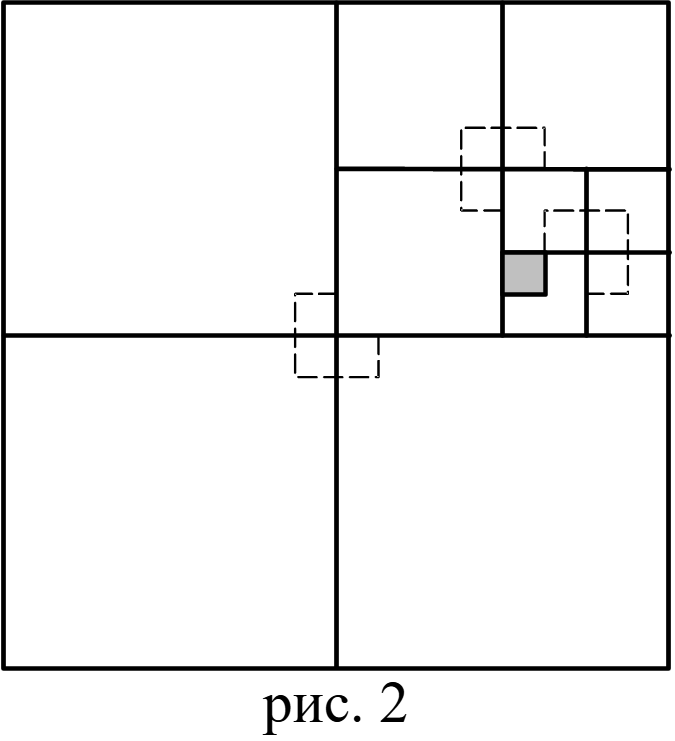
\includegraphics[scale=0.15]{./img/kvadrat2}
\end{minipage}
\hfill
\begin{minipage}{0.72\linewidth}\setlength{\parindent}{1.5em}
    Наверное, все уже поняли, что произойдёт дальше. По аналогичному сценарию мы можем разрезать на требуемые ''уголки'' и квадрат $16 \cdot 16$, и квадрат $32 \cdot 32$, и т.д. Однако мы забыли, что задача звучала несколько иначе, нежели та, которую мы пока решили, а именно: вырезается из квадрата $16 \cdot 16$ не угловая клетка, а произвольная! Что же делать? 
    \par 
    Довести полученное нами решение до искомого не так уж и трудно. Квадрат $16 \cdot 16$ делим на четыре квадрата $8 \cdot 8$, один из которых (тот, где вырезанная клетка) делим на четыре квадрата $4 \cdot 4$, один из них опять же делим на четыре квадрата $2 \cdot 2$ и начинаем вырезать ''уголки''. Сначала в том квадратике, где имеется вырезанная клетка, затем ''уголки'' от трёх
оставшихся квадратиков $2 \cdot 2$, $4 \cdot 4$ и $8 \cdot 8$ (рис. 2). 
\end{minipage}
\end{figure}}

Далее каждый из оставшихся квадратов с вырезанной угловой клеткой мы умеем разрезать на ''уголки'' из трех клеток. \qed

\textit{\textbf{Обсудим решение.}} Проследим за логикой наших рассуждений. Сначала мы существенно упростили искомую задачу (уменьшили размеры и передвинули, как захотели вырезанную клетку), затем, получив решение самой простой задачи, заметили, что при решении следующей задачи мы можем воспользоваться уже полученным результатом. Далее, как снежный ком - при решении третьей задачи пользуемся результатами второй и так можно продолжать до бесконечности. Ясно, что, идя так по цепочке, мы дойдем до каждого из её утверждений, значит все они верны. Таким образом, мы доказали даже более сильный факт, чем требовалось: любой квадрат $2n \cdot 2n$ без одной клетки можно разрезать на ''уголки'' из трех клеток.

{\setlength{\intextsep}{2pt}
\begin{figure}[h]
\begin{minipage}{0.45\linewidth}\setlength{\parindent}{1.5em}
Описанный процесс очень напоминает всем знакомую детскую игру - выстраиваешь друг за другом костяшки домино, а затем толкаешь первую. Она повалит вторую, та - третью и так до тех пор, пока не упадут все (рис. 3). Только в наших рассуждениях вместо падающих доминошек - последовательные доказательства утверждений. 
\end{minipage}
\hfill
\begin{minipage}{0.50\linewidth}
    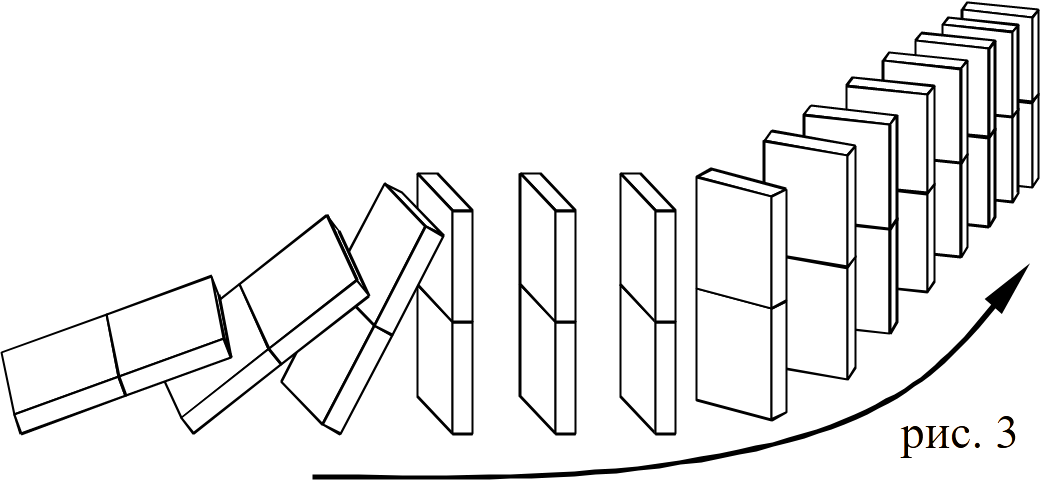
\includegraphics[scale=0.32]{img/domino.png}
\end{minipage}
\end{figure}}
Доказали одно, оно влечёт за собой доказательство следующего, следующее - дальше и т.д.\footnote{Для знатоков: это ещё не индукция в чистом виде. Это пока только рассуждения, подобные индукционным}

\begin{center}
\textbf{Основные определения.}
\end{center}

Прежде чем вводить какие-либо определения заметим, что в предыдущих рассуждениях (задача \ref{6.0 thm1}) все доказываемые утверждения были очень похожи и отличались только степенью двойки в размерах квадрата. Поэтому естественно занумеровать все эти утверждения. 
\par
Первое ($A_1$): квадрат $2^1 \cdot 2^1$ без одной клетки можно разбить на ''уголки''. 
\par
Второе ($A_2$): квадрат $2^2 \cdot 2^2$ без одной клетки можно разбить на ''уголки''. 
\par
Третье ($A_3$): квадрат $2^3 \cdot 2^3$ без одной клетки можно разбить на ''уголки''...

\begin{ex}
Сформулируйте пятое, семнадцатое и 2012-е утверждения в этой цепочке.
\end{ex}

\begin{ex}
Сформулируйте $n$-е, $(n+1)$-е и $k$-е утверждения в этой цепочке.
\end{ex}

Таким образом, можно представить, что все наши утверждения выстроились в очередь (за доказательством!) друг за другом как ''доминошки'', а мы приготовились их ''толкать''. Понятно, надо убедиться, что падая, каждая заденет и увлечёт за собой следующую.

\newpage

\textbf{Основная схема.} Изложенный выше метод рассуждений требует установления истинности двух фактов:

\fbox{\begin{minipage}{0.95\textwidth}
    \textbf{\textit{Факт 1.}} Первое утверждение верно. (мы можем толкнуть первую доминошку)
    \par
    \textbf{\textit{Факт 2.}} Если интересующее нас утверждение верно на каком-то шаге, то верно и следующее за ним утверждение. (толкнув одну, уроним и следующую)
\end{minipage}} 

Первый факт называется \textit{базой (базисом) индукции}, второй - \textit{индукционным переходом} или \textit{шагом индукции}. Индукционный переход включает в себя \textit{посылку (предположение) индукции} (утверждение верно при $n = k$) и \textit{заключение} (утверждение верно при $n = k + 1$). Другими словами, шаг индукции состоит в переходе от посылки к заключению, т.е. в выводе, что заключение верно, если верна посылка. (если упадет $k$-я
доминошка, то упадет и $(k+1)$-я) 

Итак, пусть имеется последовательность утверждений: $A_1$, $A_2$, $...$, $A_n$, $...$ . Для того, чтобы доказать
справедливость \textit{\underline{всех}} утверждений этой последовательности, можно поступить следующим образом:
\begin{enumerate}
\item Доказать истинность утверждения $A_1$;
\item Доказать, что при \textit{\underline{любом}} натуральном $n$ из справедливости утверждения $A_n$ следует справедливость
утверждения $A_n+1$. 
\end{enumerate}

Логический приём, позволяющий заключить, что рассматриваемое утверждение верно для всех натуральных чисел, коль скоро справедливы и базис, и переход называется \textit{методом математической индукции} (ММИ). Утверждения $A_1, A_2, A_3, ...$ называют частными формулировками, а утверждение ''для всякого $n$ имеет место $A_n$'' - универсальной формулировкой. Если мы доказали и базу, и переход, то истинность универсальной формулировки основана на следующем стандартном рассуждении:

\fbox{\begin{minipage}{0.95\textwidth}
    Утверждение $A_1$ истинно, т.к. мы доказали базу индукции. Последовательно применяя индукционный переход при $k=1, 2, 3, ...$ , получаем истинность утверждений $A_2, A_3, A_4, ...$ . Этим способом мы можем последовательно дойти до любого значения $n$ и убедиться, что это $A_n$ истинно. Следовательно, для всякого $n$ утверждение $A_n$ справедливо.
\end{minipage}} 

Таким образом, метод математической индукции заключается, по существу, в разрешении не пользоваться стандартным рассуждением в каждой конкретной ситуации, т.е. он позволяет сделать заключение об истинности универсальной формулировки сразу, как только установлена истинность базиса индукции и индукционного перехода.

\section{Доказательство числовых тождеств.}
\epigraph{\textit{''Все равны! Ибо равенство ещё не тождество!''}}{\textit{Афоризм неизвестного автора.}}

\begin{thm}
    Докажите, что при любом натуральном $n$ справедливо равенство 

    $$1 + 2 + 3 + ... + n = \dfrac{n(n+1)}{2}$$
\end{thm}

\begin{prf}
У нас имеется последовательность утверждений:
\par
$A_1 : 1 = \dfrac{1 \cdot 2}{2}$;
\hfill
$A_2 : 1 + 2 = \dfrac{2 \cdot 3}{2}$;
\hfill
$A_3 : 1 + 2 + 3  = \dfrac{3 \cdot 4}{2}$;
\hfill
...
\par
1. \textit{\underline{База индукции:}} очевидно, что утверждение $A_1$ верно.
\par
2. \textit{\underline{Индукционный переход:}} пусть утверждение верно для $n = k$, или, другими словами, пусть верно какое-то
утверждение $A_k$, т.е. верно равенство 1 + 2 + 3 + ... + $k$ = $\dfrac{k(k+1)}{2}$ (предположение, что $A_k$ верно называется
\textit{индукционным предположением}). Докажем, что тогда утверждение верно и для $n = k +1$, т.е. верно утверждение $A_{k+1}$. Для этого добавим к обеим частям $A_k$ по ($k + 1$):

$$1 + 2 + 3 + ... + k + (k + 1) = \dfrac{k(k+1)}{2} + (k + 1) = \dfrac{k(k+1)}{2} + \dfrac{2(k+1)}{2} = \dfrac{(k+1)(k+2)}{2}$$

Но это как раз и есть утверждение $A_{k+1}$. В силу принципа математической индукции верны все утверждения
$A_1$, $A_2$, ... , т.е. наша формула верна при любом натуральном $n$.
\end{prf}

\par

\textbf{\textit{Замечание 1.}} Обращаем ваше внимание, что при выполнении индукционного перехода важно показать, что
все проводимые рассуждения справедливы для любого $k$.

\textbf{\textit{Замечание 2.}} Вместо утверждения $A_1$ в качестве базы индукции мы могли взять, например, утверждение $A_5$. Тогда, выполнив индукционный переход, мы бы доказали, что исходное утверждение верно для всех натуральных $n$, начиная с 5.\footnote{Заметим, что тогда справедливость утверждений 1, 2, 3, 4 мы не доказали и ничего про них не знаем. Такая индукция имеет смысл, если для меньших значений $n$ утверждение не определено. Например, в задачах про многоугольники число сторон не может быть меньше 3, поэтому нет смысла рассматривать утверждения для ''двуугольников'' или
''одноугольников''.}

\begin{thm}
Докажите, что сумма углов выпуклого $n$-угольника равна $180 ^{\circ} \cdot (n-2)$.
\end{thm}

\begin{prf}
Утверждение задачи имеет смысл при всех натуральных $n \geq 3$, поэтому и базой индукции будет соответственно $n = 3$.
\par
\textit{\underline{База}}: утверждение $A_3$ верно по теореме о сумме углов треугольника.
\par
\textit{\underline{Переход}}. выведем заключение о том, что ''сумма углов выпуклого ($k$ + 1)-угольника равна $180 ^{\circ} \cdot ((k + 1) - 2) = 180 ^{\circ} \cdot (k -1)$'' из предпосылки ''сумма углов выпуклого $k$-угольника равна $180 ^{\circ} \cdot (k - 2)$''. Для этого в $(k + 1)$-угольнике возьмём две вершины по разные стороны от какой-либо вершины, и соединим их диагональю (это всегда возможно ввиду выпуклости многоугольника)\footnotemark
\end{prf}
\footnotetext{Существует несколько определений выпуклого многоугольника. В данном случае можно использовать любое из двух: 
    \par
    Первое - ''многоугольник называется выпуклым, если для любых двух его точек $A$ и $B$ отрезок $AB$ целиком принадлежит этого многоугольнику''. (аналогичным образом можно дать определение любой выпуклой фигуры)
    \par
    Второе - ''многоугольник называется выпуклым, если любая диагональ принадлежит ему целиком'', которая разобьёт исходный многоугольник на две части: на треугольник и выпуклый $k$-угольник. Сумму углов исходного многоугольника можно получить, сложив сумму углов треугольника ($180 ^{\circ}$) и сумму углов $k$-угольника $(180 ^{\circ} (k-2)$ - индукционное предположение!). Складывая эти суммы, получаем $180 ^{\circ} (k-1)$, что и требовалось доказать.}
    
\section{Задачи на делимость.}

Техника составления и обоснования индукционных переходов при решении задач на делимость похожа на соответствующую технику для тождеств: для доказательства обычно выясняется, КАК изменяется выражение при переходе от $k$ к $k + 1$ и проверяется делимость этого ''изменения'' на нужное число.

\begin{thm}
Докажите, что $n^3 + (n + 1)^3 + (n+2)^3$ делится на 9 при любом натуральном $n$.
\end{thm}

\begin{prf}
Утверждение задачи имеет смысл при всех натуральных $n \geq 3$, поэтому и базой индукции будет соответственно $n = 3$.
\par
\textit{\underline{База}}: $(n = 1)$: $1^3 + 2^3 + 3^3 = 36$ - делится на 9.
\par
\textit{\underline{Переход}}. пусть при $n = k$ утверждение задачи
истинно (т.е. $k^3 + (k + 1)^3 + (k + 2)^3 \del 9$ при некотором $k$). Докажем тогда, что при $n = k + 1$ утверждение также
справедливо (т.е. $(k + 1)^3 + (k+2)^3 + (k+3)^3 \del 9)$. В самом деле,
$$(k + 1)^3 + (k + 2)^3 + (k + 3)^3 = \underbrace{(k + 1)^3 + (k + 2)^3 + k^3}_{\mathclap{\del\text{9 по предположению индукции}}} + \underbrace{9k^2 + 27k + 27}_{очевидно \del 9}$$
а сумма двух чисел, кратных 9, также кратна 9, что и требовалось доказать.
\par
Тем самым переход доказан и всё утверждение доказано.
\end{prf}

\newpage

\begin{thm}
Докажите, что $47^n + 22$ кратно 23 при любом натуральном $n$.
\end{thm}

\begin{prf}
\par
\textit{\underline{База}} $(n = 1)$: 47 + 22 = 69 - делится на 23. 
\par
\textit{\underline{Переход}}. Пусть при $n = k$ утверждение задачи истинно (т.е. $47^k + 22 \del 23$ при некотором $k$). Докажем тогда, что при $n = k + 1$ утверждение также справедливо (т.е. что $47k + 1
+ 22 \del 23$). В самом деле,
$$47^{k+1} + 22 = 47^k \cdot 47 + 22 \cdot 47 - 22 \cdot 47 + 22 = 47 \cdot \underbrace{(47^k + 22)}_{\mathclap{\del\text{23 по предположению индукции}}} - \overbrace{(22 \cdot 46)}^{очевидно \del 23}$$
а разность двух чисел, кратных 23, также кратна 23, что и требовалось доказать.
\par
Тем самым переход доказан и всё утверждение доказано.
\end{prf}

\vspace*{\fill}

\textbf{\textit{Замечания к листку.}}
\par
Метод математической индукции является серьёзным инструментом для решения задач. Как и любой инструмент перед применением он требует подготовки. В данном конкретном случае подготовка будет заключаться в произнесении ''стишка'', посвященного ММИ. Помните, что прежде чем начать рассуждение,
вы должны сообщить, по какой переменной вы будете вести индукцию, например, так:
\\
''Будем доказывать методом математической индукции \textit{по n} или \textit{по числу переменных} или \textit{по количеству треугольников} или ...'' Далее вы обязаны указать Базу и доказать её. Затем сформулировать индукционное предположение и переход, который собираетесь доказать. Потом доказать переход и завершить доказательство изящной фразой: ''Тем самым переход доказан и всё утверждение доказано''.

\newpage

\begin{thm}
Докажите, что число 111...11 (243 единицы) делится на 243.
\end{thm}

\begin{prf}\footnote{Заметим, что при решении аналогичных задач возникают типичные ошибки: признака делимости на 27, аналогичного признакам делимости на 3 и на 9 - нет; если число делится на 3 и на 9, то совсем не обязательно, что оно делится на 27.}
Будем доказывать общее утверждение, а именно, что число, записываемое $3^n$ единицами, делится на $3^n$. Индукция по показателю $n$.
\par
\textit{\underline{База}}: 111 делится на 3.  
\par
\textit{\underline{Индукционное предположение}}. Пусть верно для $n = k$, т.е. верно, что число, записываемое $k$ единицами, делится на $3^k$.
\par
\textit{\underline{Переход}}. Докажем для $n = k + 1$. Разделим число, записанное $3^{k+1}$ единицами на число, записанное $3^k$ единицами. Получим число 100..010..01 (две последовательности нулей по $3^k$ - 1 штук). Очевидно, что полученное число делится на 3. Следовательно, исходное число делится на $3^{k+1}$ и тем самым индукционный переход, а, значит, и всё утверждение, доказаны. В частности оно доказано для $n = 5$, поэтому доказано требуемое утверждение, т.к. $243 = 3^5$.
\end{prf}

В предыдущей задаче был осуществлён характерный приём при доказательстве с помощью метода математической индукции, а именно - \textit{обобщение утверждения}. Вместо конкретного утверждения, для конкретного значения длины, количества и т.п. доказывается утверждение \textit{в общем виде}, а требуемое утверждение является частным случаем доказанного. Аналогичный приём был осуществлён в самой первой задаче про разрезание клетчатой доски.

\begin{thm}
В прямоугольнике $3 \cdot 2011$ (2011 столбцов и 3 строки) стоят фишки 3 цветов, по 2011 каждого цвета. Докажите, что можно переставить в каждой строке фишки так, чтобы в каждом столбце были фишки всех трёх цветов.
\end{thm}

{\setlength{\intextsep}{2pt}
\begin{figure}[h]
\begin{minipage}{0.65\linewidth}\setlength{\parindent}{1.5em}
\begin{thm}
На фестивале военно-морской песни собрались 100 хоровых коллективов из разных стран. Каждый хор поёт три песни подряд и тут же уезжает. Жюри, ознакомившись с текстами, выяснило, что каждая песня оскорбительна ровно для одной из стран-участниц. Докажите, что можно составить их расписание выступлений так, чтобы никому не пришлось выслушивать более трех оскорбительных для него песен.
\end{thm}
\end{minipage}
\hfill
\begin{minipage}{0.30\linewidth}
    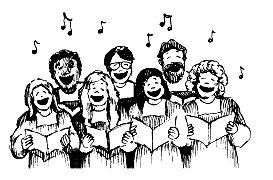
\includegraphics[width=0.95\columnwidth]{img/hor.png}
\end{minipage}
\end{figure}}

\begin{thm}$^{\ast}$
Докажите, что существует 100-значное число, делящееся на 2100, в десятичной записи которого участвуют только цифры 1 и 2.
\end{thm}

\begin{thm}$^{\ast}$
На доске в строчку написаны 100 цифр - нули и единицы (в любой комбинации). Разрешается выполнять два действия: 1) заменять первую цифру (нуль на единицу и единицу на нуль), 2) заменять цифру, стоящую после первой единицы. (Пример: в последовательности 0001101... можно заменить подчёркнутые цифры) Докажите, что с помощью конечного числа таких замен можно получить любую наперёд заданную комбинацию нулей и единиц. 
\end{thm}

\begin{thm}
    Имеется 2011 квадратов. Докажите, что их можно разрезать на части, из которых сложится один квадрат.
\end{thm}

\section{Неравенства.}
\epigraph{\textit{''Равенство двух неравенств возможно только в том случае, когда неравенства идентичны.''}}{Афоризм неизвестного автора.}

Приёмы доказательств неравенств более разнообразны, однако, наиболее часто используется следующий факт ''сложения неравенств'': если $a>b$ и $c > d$, то $a + c > b + d$. Здесь в роли неравенства $a$ > $b$ выступает неравенство для $k$, а $c$ и $d$ - ''довески''~к левой и правой частям соответственно при переходе от $k$ к $k + 1$. Кроме того, часто используются промежуточные неравенства. т.е. если нужно доказать, что $A>B$, то доказывают, что $A>C$, а затем пользуются тем, что $C>B$.

\begin{thm}
Докажите, что модуль суммы любого числа слагаемых не превосходит суммы модулей этих слагаемых.
\end{thm}

\begin{thm}
Докажите, что при любом натуральном $n$ справедливо неравенство $2^n > n$.


\end{thm}

\begin{prf}
\par
\textit{\underline{База}}: $n = 1$. $2^1 > 1$ - верно.
\par
\textit{\underline{Переход}}. Пусть доказано для $n = k$, т.е. (\textit{\underline{индукционное предположение}}) пусть верно \begin{equation} \label{eq_6_5}
    2^k > k
\end{equation} 
Докажем для $n = k + 1$, т.е. докажем, что тогда верно $2^{k+1} > k + 1$.
\par
\textit{1 способ.} Умножим обе части верного по предположению неравенства \ref{eq_6_5} на 2, получим верное неравенство $2k+1 > 2k$. Но для любого натурального $k$ выполняется $2k \geq k + 1$, следовательно, верно, что  $2k + 1 > k + 1$.
\par
\textit{2 способ.} Воспользуемся неравенством, верным для любого натурального $k$ выполняется $2k$ > 1. Прибавим к этому неравенству верное по предположению неравенство \ref{eq_6_5}. Получим $2k + 2k > k + 1$. Но выражение в правой части равно $2k + 1$, следовательно, доказано утверждение для $n = k + 1$.
\par
Тем самым переход доказан и всё утверждение доказано. 
\end{prf}

\begin{thm}$^n$ \label{6.0 n1}
Докажите, что при любом натуральном $n$ справедливо неравенство $3n > n + 1$. 
\end{thm}

\begin{thm}
При каких натуральных $n$ выполнено:~а)~$2n > 2n + 1$;~б)~$2n > n^2$~?
\end{thm}

\begin{thm}$^n$ \label{6.0 n2}
Докажите, что при любом натуральном $n$ справедливо неравенство $\dfrac{(2n)!}{(n!)^2} > \dfrac{4^n}{n+1}$
\end{thm}

\begin{thm}$^\ast$
Докажите, что при любом натуральном $n$, начиная с 2, справедливо неравенство: 	
$$2^n > 1 + n \sqrt{2^{n-1}}$$\end{thm}

\begin{thm}
Докажите, что при любом натуральном $n$, начиная с 2, справедливо неравенство: 
    $$\dfrac{1}{n + 1} + \dfrac{1}{n+2} + ... + \dfrac{1}{2n} > \dfrac{13}{14}$$
\end{thm}

\begin{thm}
Докажите \textit{неравенство Бернулли}: $(1 + x)^n \geq 1 + nx$ при $x \geq -1, n \in \mathbb{N}$.
\end{thm}

\begin{thm}
Докажите, что при любом натуральном $n$ справедливо неравенство $$1 + \dfrac{1}{2} + \dfrac{1}{4} + ... + \dfrac{1}{2^n} < 2$$
\end{thm}

\begin{prf} Докажем неравенство индукцией по $n$.
\par
\textit{\underline{База}}: $(n = 1)$. $1 + \dfrac{1}{2} < 2$ верно.
\par
\textit{\underline{Индукционное предположение}}. Пусть верно для $n = k$, т.е. верно, что 
\begin{equation} \label{eq_6_1}
    1 + \dfrac{1}{2} + \dfrac{1}{4} + ... + \dfrac{1}{2^k} < 2
\end{equation}
\par
\textit{\underline{Переход}}. Докажем для $n = k + 1$, т.е. докажем, что тогда верно
\begin{equation} \label{eq_6_2}1 + \dfrac{1}{2} + \dfrac{1}{4} + ... + \dfrac{1}{2^k} + \dfrac{1}{2^{k+1}} < 2
\end{equation}
Разделим обе части неравенства (\ref{eq_6_1}) на 2. Получим: $\dfrac{1}{2} + \dfrac{1}{4} + ... + \dfrac{1}{2^k} + \dfrac{1}{2^{k+1}} < 1$. Прибавляя к обеим частям этого неравенства по 1, получаем неравенство (\ref{eq_6_2}). Тем самым переход доказан и требуемое неравенство доказано. 
\end{prf}

\newpage

\section{Парадокс изобретателя.}

{\setlength{\intextsep}{2pt}
\begin{figure}[h]
\begin{minipage}{0.74\linewidth}\setlength{\parindent}{1.5em}
Попробуем доказать при помощи метода математической индукции два неравенства:
\par
\begin{equation*}
  1)~\dfrac{1}{2} \cdot \dfrac{3}{4} \cdot ... \cdot \dfrac{2n - 1}{2n} < \dfrac{1}{\sqrt{n}} ~~~и~~~
  2)~\dfrac{1}{2} \cdot \dfrac{3}{4} \cdot ... \cdot \dfrac{2n - 1}{2n} < \dfrac{1}{\sqrt{n + 1}}
\end{equation*}

\par
Базис индукции проверяется без труда
\begin{equation*}
  1)~ \dfrac{1}{2} < \dfrac{1}{1} = \dfrac{1}{\sqrt{1}} ~~~и~~~   
  2)~ \dfrac{1}{2} < \dfrac{1}{\sqrt{2}} = \dfrac{1}{\sqrt{1 + 1}}
\end{equation*}
\par
По предположению индукции, мы имеем
\begin{equation*}
  1)~\dfrac{1}{2} \cdot \dfrac{3}{4} \cdot ... \cdot \dfrac{2k + 1}{\sqrt{2k + 2}} = \dfrac{1 \cdot 3 \cdot ... \cdot (2k - 1)}{2 \cdot 4 \cdot ... \cdot 2k} \cdot \dfrac{2k + 1}{2k + 2} < \dfrac{1}{\sqrt{k}} \cdot \dfrac{2k + 1}{2k + 2}
\end{equation*}
$$и$$
\begin{equation*}
  2)~\dfrac{1}{2} \cdot \dfrac{3}{4} \cdot ... \dfrac{2k + 1}{\sqrt{2k + 2}} = \dfrac{1 \cdot 3 \cdot ... \cdot (2k - 1)}{2 \cdot 4 \cdot ... \cdot 2k} \cdot \dfrac{2k + 1}{2k + 2} < \dfrac{1}{\sqrt{k + 1}} \cdot \dfrac{2k + 1}{2k + 2}
\end{equation*}

\end{minipage}
\hfill
\begin{minipage}{0.25\linewidth}
    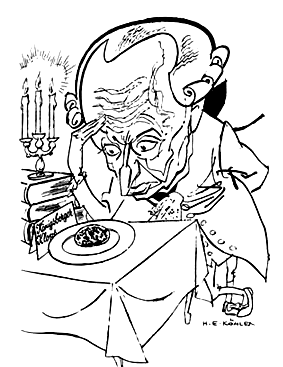
\includegraphics[width=0.95\columnwidth]{img/euler_k.png}
\end{minipage}
\end{figure}}

\par
нам остаётся доказать, что
\begin{equation*}
1)~\dfrac{1}{\sqrt{k}} \cdot \dfrac{2k + 1}{2k + 2} \leq \dfrac{1}{\sqrt{k + 1}}
   ~~~и~~~    
  2)~\dfrac{1}{\sqrt{k + 1}} \cdot \dfrac{2k + 1}{2k + 2} \leq \dfrac{1}{\sqrt{k + 2}}
\end{equation*}

\par
Возводя обе части неравенства в квадрат, избавляясь от знаменателей и раскрывая скобки, 
\par
приходим к эквивалентным неравенствам
\begin{equation*}
1)~4k^3 + 8k^2 + 5k + 1 \leq 4k^3 + 8k^2 + 4k
 ~~~и~~~
  2)~4k^3 + 12k^2 + 9k + 2 \leq 4k^3 + 12k^2 + 12k + 4
\end{equation*}

Вспоминая, что число $k$ натуральное, легко убедиться, что левое неравенство неверно, а правое верно. Но как же так оказалось? Ведь правое неравенство сильнее (!), и из него автоматически следует левое. Дело в том, что хотя во втором случае нам и пришлось доказывать более сильное заключение, но одновременно с этим мы могли пользоваться и более сильным предположением индукции. При этом, ни в коем случае нельзя считать первое неравенство неверным. Наша неудача в нём говорит лишь о том, что не годится конкретный метод доказательства - математическая индукция. 
\par
Подобная ситуация получила название \textit{парадокс изобретателя}.\footnote{На рисунке приведена карикатура на Иммануила Канта (1724 - 1804). Современные кенигсбержцы достаточно хорошо знают великого земляка Иммануила Канта. Он известен как философ и как профессор Кенигсбергского университета, написавший большое количество философских работ, в том числе изданную на русском языке ''Критику чистого разума''.
Но Кант известен не только как философ и преподаватель, но и как простой человек, имеющий свои слабости. Известен он также и как педант, как человек, не покидавший Кенигсберг всю свою жизнь и дальше его окрестностей не выезжавший. Но мало кто знает, что он еще прославился и как изобретатель, достигнув высот, которые если не уравнивают его с Леонардо да Винчи, то, по крайней мере, ставят его в один ряд со многими изобретателями мирового значения. Кто бы мог предположить, что такой обыденный канцелярский прибор, как дырокол впервые был придуман и использован Кантом. Единственное отличие от современного дырокола, имеющего отверстие 5 мм, является то, что Кант использовал аналогичный прибор с отверстием 11,6 мм. По этому диаметру отверстия всегда можно определить дырокол, изобретенный Кантом. До середины 19 века не было документов, которые имели бы такие аккуратные отверстия, кроме документов Иммануила Канта. Первые листы, подшитые к делу с отверстием 11,6 мм, обнаружили советские исследователи в 1956 году. Они датировались декабрем 1799 г., и эта дата была объявлена датой первого употребления дырокола, изобретенного Кантом. Но через пять лет уже в Германии были обнаружены бумаги Канта с отверстием диаметром 11,6 мм за октябрь 1787 г. И дата первого употребления дырокола в канцелярском мире сдвинулась на 12 лет...
\par
При опросе работников канцелярий оказалось, что 75\% из них знают Иммануила Канта только как изобретателя дырокола; 5\% - что он еще является философом, и 2\% - что он еще преподавал в Кенигсбергском университете. Остальные 18\% вообще ничего не слышали о Канте. \smiley}

\par
Парадокс изобретателя предложил нам ещё одну идею доказательства неравенств, а именно - усиление утверждения. Примером такого метода может служить задача: ''Докажите неравенство $\dfrac{1}{2} \cdot \dfrac{3}{4} \cdot ... \cdot \dfrac{2n - 1}{2n} < \dfrac{1}{\sqrt{n}}$.'' Вместо доказательства требуемого неравенства мы доказываем по индукции более сильное неравенство $\dfrac{1}{2} \cdot \dfrac{3}{4} \cdot ... \cdot \dfrac{2n - 1}{2n} < \dfrac{1}{\sqrt{n + 1}}$.'', а затем пользуемся тем, что $\dfrac{1}{\sqrt{n+1}} < \dfrac{1}{\sqrt{n}}$.

\newpage

Разберём еще один пример.

\begin{thm}
Докажите, что при любом натуральном n справедливо неравенство \par $1 + \dfrac{1}{2} + \dfrac{1}{4} + ... + \dfrac{1}{2^n} < 2$.
\end{thm}

\begin{prf}
Сначала усилим наше утверждение и рассмотрим равенство $1 + \dfrac{1}{2} + \dfrac{1}{4} + ... + \dfrac{1}{2^n} = 2 - \dfrac{1}{2^n}$. Теперь это равенство будем доказывать индукцией по $n$.
\par
\textit{\underline{База}}: $n$ = 1. $1 + \dfrac{1}{2} = 2 - \dfrac{1}{2}$ верно.
\par
\textit{\underline{Индукционное предположение}}. Пусть верно для $n = k$, т.е. верно, что
\begin{equation} \label{eq_6_3}
    1 + \dfrac{1}{2} + \dfrac{1}{4} + ... + \dfrac{1}{2^k} = 2 - \dfrac{1}{2^k}.
\end{equation}

\par

\textit{\underline{Переход}}. Докажем для $n = k + 1$, т.е. докажем, что тогда верно
\begin{equation} \label{eq_6_4}
1 + \dfrac{1}{2} + \dfrac{1}{4} + ... + \dfrac{1}{2^k} + \dfrac{1}{2^{k + 1}} = 2 - \dfrac{1}{2^{k + 1}}.
\end{equation}

Для доказательства этого факта прибавим к каждой части верного по предположению равенства (\ref{eq_6_3}) дробь $\dfrac{1}{2^{k+1}}$. Получим:
$$
    1 + \dfrac{1}{2} + \dfrac{1}{4} + ... + \dfrac{1}{2^k} + \dfrac{1}{2^{k + 1}} = 2 - \dfrac{1}{2^k} - \dfrac{1}{2^{k + 1}}.
$$

В левой части мы имеем в точности левую часть доказываемого равенства (\ref{eq_6_4}), а в правой: 
$$
    2 - \dfrac{1}{2^k} + \dfrac{1}{2^{k + 1}} = 2 - 2 \times \dfrac{1}{2^{k + 1}} + \dfrac{1}{2^{k + 1}} = 2 - \dfrac{1}{2^{k + 1}}
$$
, что есть правая часть неравенства (\ref{eq_6_4}). Тем самым переход доказан и усиленное утверждение доказано. Но раз верно более сильное утверждение, то верно и исходное неравенство. \end{prf}

\begin{thm} $^*$
Докажите, что при любом натуральном $n$ справедливо неравенство \par $1 + \dfrac{1}{4} + \dfrac{1}{9} + ... + \dfrac{1}{n^2} < 2$.
\end{thm}

{\setlength{\intextsep}{2pt}
\begin{figure}[h]
\begin{minipage}{0.74\linewidth}\setlength{\parindent}{1.5em}
\begin{thm} $^*$
На краю пустыни имеется неограниченный склад продовольствия и воды. Путешественник может нести на себе запас еды и питья на неделю (7 дней). Он может в любом месте пустыни делать свой склад еды и питья на сколько угодно дней (считается, что запасы не
пропадают и не портятся). Докажите, что путешественник
сможет пересечь пустыню.\footnotemark
\end{thm}
\end{minipage}
\hfill
\begin{minipage}{0.25\linewidth}
    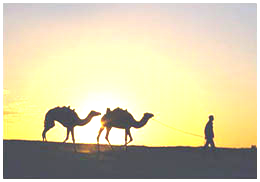
\includegraphics[width=0.95\columnwidth]{img/camels.png}
\end{minipage}
\end{figure}}\footnotetext{Для программистов. В 2002 году на студенческом кубке мира по программированию была задача ''Пересечение пустыни'': ''Вам предстоит пеший поход через пустыню между двумя заданными её точками. В начальной точке путешествия вы можете запастись провизией и неограниченным количеством воды. В разных местах пустыни могут находиться оазисы, где вы можете восполнить запасы воды, а также оставить часть провизии на хранение. На прямоугольной карте пустыни ваш маршрут задаётся координатами его начальной и конечной точек, а также мест, где
расположены оазисы, при этом шаг координатной сетки равняется одной миле. Во время путешествия провизию и воду вы тратите, не отдыхая в оазисах, а синхронно продвижению по маршруту (по единице веса на каждую милю). Хотя в конечную точку маршрута можно прийти налегке, в случае досрочного окончания запасов дальнейшее продвижение по пустыне невозможно. Разумеется, предельный суммарный вес провизии и воды, который вы способны нести, ограничен; приобрести на старте более миллиона весовых единиц еды вам также не удастся. В качестве исходных данных известны координаты начальной и конечной точек маршрута, всех оазисов, а также максимальный вес груза, который вы способны нести. Необходимо определить, возможен ли переход, отвечающий заданным условиям, и если да, то каким запасом провизии необходимо для него запастись.'' Что называется - найдите 10 отличий \smiley}

\newpage

\section{Математическая индукция и догадка по аналогии.}

{\setlength{\intextsep}{2pt}
\begin{figure}[h]
\begin{minipage}{0.64\linewidth}\setlength{\parindent}{1.5em}
Иногда встречаются задачи, в которых нет очевидной формулы
для $n$-го утверждения. Её придётся сначала придумать, а затем
ещё и доказать. Возникает вопрос: как придумать? Для этого
обычно рассматривают несколько частных случаев и на их
основании пытаются вывести общую формулу.
\end{minipage}
\hfill
\begin{minipage}{0.35\linewidth}
    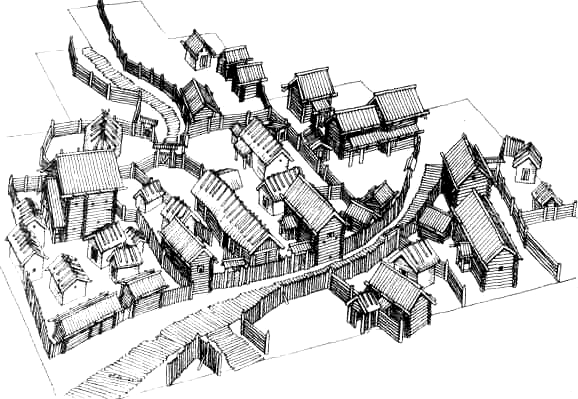
\includegraphics[width=0.95\columnwidth]{img/city.png}
\end{minipage}
\end{figure}}

\begin{thm}
На сколько частей делят плоскость $n$ прямых, среди которых нет параллельных и никакие три не пересекаются в одной точке?\footnotemark
\end{thm}\footnotetext{Такие прямые называются прямыми общего положения.}

\begin{prf}
    Обозначим через $A_n$ количество частей, на которые делят плоскость $n$ прямых. Найдём несколько значений $A_n$ при небольших значениях $n$ вручную:
    \par
    $A_0 = 1, A_1 = 2, A_2 = 4, A_3 = 7, A_4 = 11$. \underline {Ага!} $A_1 = A_0 + 1, A_2 = A_1 + 2, A_3 = A_2 + 3, A_4 = A_3 + 4$.
    \par
    Похоже, что $A_n = 1 + (1 + ... + n)$, но это пока лишь догадка, основанная на предположении, что добавление $n$-ой прямой увеличивает число частей на $n$. Итак, мы сформулировали гипотезу, которую попытаемся сейчас доказать с помощью индукции.  
    
    \textit{\underline{База}}. Для $n = 0$ (прямых не проведено). Число кусков - 1. Верно.
    \par
    \textit{\underline{Переход}}. Пусть доказано для количества кусков $A_k$, тогда $k$ прямых общего положения разбивают плоскость на $1 + \dfrac{k(k + 1)}{2}$ частей. Докажем, что тогда $A_{k+1} = 1 + \dfrac{(k + 1)((k + 1) + 1)}{2} = 1 + \dfrac{(k + 1)(k + 2)}{2}$. Пусть проведена $k + 1$ прямая. Выберем любую прямую и временно удалим её из рассмотрения... Тогда оставшиеся $k$ прямых разбивают плоскость на $1 + \dfrac{k(k + 1)}{2}$ частей. Вновь проведём $(k + 1)$-ю прямую. Эта прямая пересекает старые прямые в $k$ точках (прямых $k$ и с каждой пересекается) и, значит, рассекает $k + 1$ старых кусков. 
    Следовательно, $A_{k + 1} = A_k + k + 1 = 1 + \dfrac{k(k + 1)}{2} + k + 1 = 1 + \dfrac{k(k + 1) + 2(k + 1)}{2} = 1 + \dfrac{(k + 1)(k + 2)}{2}$. 
    \par
    Наша гипотеза доказана.
    \par
    \textit{\underline{Ответ}}: $1 + \dfrac{n(n + 1)}{2}$. \end{prf}

\begin{thm}
    На какое число частей могут разбивать плоскость $n$ равносторонних не пересекающихся треугольников?
\end{thm}

\begin{thm}\label{thm6_1}
    В городе Заборске $N$ домов. Какое наибольшее число заборов можно построить в этом городе, если по приказу мэра должны выполняться следующие условия:
    \par
        1) заборы не должны пересекаться;
        \par
        2) каждый забор ограничивает хотя бы один дом;
        \par
        3) никакие два забора не ограничивают один и тот же набор домов?
\end{thm}

\textbf{\textit{Замечание 3.}} Отметим, что рассуждения ''по аналогии'' не всегда подсказывают верную формулу. Наиболее
известным является пример Леонарда Эйлера:
\par
\textit{Верно ли, что число $n^2 + n + 41$ - простое при любом натуральном $n$?}\footnote{В XVIII веке многие математики были увлечены идеей поиска формулы простых чисел. Как раз в это время и была предложена данная формула, которая, однако, не оправдала надежд.}
\par
Кажется, что это действительно так. ''Экспериментируя'' с небольшими значениями $n$, можно обнаружить, что при всех $n$ от 1 до 39 получаются простые числа. Но: $402 + 40 +4 1 = 412$ или $412 + 41 + 41 = 41 \times 43$.

\newpage

\begin{thm} $^*$
На доске написаны два числа 1, 1. Впишем между ними их сумму: 1, 2, 1. Повторим операцию: 1, 3, 2, 3, 1. После трёх операций на доске будет написано 1, 4, 3, 5, 2, 5, 3, 4, 1. Какова будет сумма всех чисел после 100 таких операций? 
\end{thm}

\newpage

\section{Другие схемы индукции.}

\epigraph{\textit{Бэкон\footnotemark выдвинул новаторскую идею, в
соответствии с которой главным методом познания должна стать индукция.}}{Из учебника философии для студентов.}\footnotetext{Фрэнсис Бэкон (1561 - 1626) считается основателем эмпирического (опытного) направления в философии - английский философ и политический деятель (в 1620 - 1621 гг. — лордканцлер Великобритании, второе должностное лицо в стране после короля)}
До раздела ''догадки по аналогии'' при доказательстве индукционного перехода требовалась истинность только одного (предыдущего по номеру) утверждения. Исключение составляет только задача \ref{thm6_1}, но о геометрических задачах мы поговорим позже.
\par
Мы уже говорили, что иногда предположения об истинности одного утверждения недостаточно и требуется предположение об истинности сразу нескольких утверждений. Посмотрим, как изменится схема метода математической индукции в этом случае:
\par
1) \textit{\underline{База индукции}}. Доказываем истинность утверждения $A_p$;
\par
2) \textit{\underline{Индукционное предположение}}. Пусть справедливы все утверждения $A_p, A_{p+1}, ..., A_n$.
\par
3) \textit{\underline{Индукционный переход}}. Пользуясь индукционным предположением доказываем, что тогда справедливо утверждение $A_{n + 1}$.
\par
Безусловно, такой способ доказательства правомерен, ибо если волна доказательства дошла до $A_k$, то она до этого прошла и все предшествующие утверждения цепочки. При сохранении обычной базы переход в этом случае будет выглядеть так: ''При любом натуральном $k$ из истинности утверждений $A_1, A_2, ..., A_k$ вытекает истинность $A_{k + 1}$''. Примером такой задачи, где для доказательства перехода требуется истинность всех предыдущих утверждений, может служить задача \ref{thm6_1}. Разберём ещё один пример.

\begin{thm}
Докажите, что любое натуральное число можно представить в виде суммы нескольких различных степеней двойки (возможно, включая нулевую).
\end{thm}

\begin{prf}
Пусть наше натуральное число равно $n$. Докажем утверждение индукцией по $n$. 
\par
\textit{\underline{База}}: если $n$ равно 1 или 2, то представление очевидно: $1 = 2^0, 2 = 2^1$. 
\par
\textit{\underline{Индукционное предположение}}. Пусть верно для всех $n < k$, докажем для $n$, равного $k$. 
\par
\textit{\underline{Переход}}. Рассмотрим максимальную степень двойки, не превосходящую $n$. Тогда $2^m \leq k < 2^{m + 1}$. Пусть $A = k - 2^m$. Очевидно, что $0 \leq A < k$. Тогда по индукционному предположению $A$ можно представить в виде суммы различных степеней двоек (если $A$ равно нулю, то $k$ = $2^m$ и представление найдено). Но кроме того $A < 2^m$. Это значит, что в представлении $A$ эта степень двойки не участвует. Поэтому $k = 2^m + A$ даёт нам искомое представление. Тем самым переход доказан и требуемое утверждение доказано. 
\end{prf}

\begin{thm}
Докажите, что любое натуральное число можно представить в виде суммы нескольких степеней тройки (возможно, включая нулевую), где каждая степень встречается не более двух раз.
\end{thm}

\begin{thm}
Михаил Владимирович выписал в строчку 100 чисел и расставил между ними знаки арифметических действий. Витя расставляет скобки по правилам арифметики. Какое максимальное количество пар скобок он сможет расставить?
\end{thm}

В предыдущих трёх задачах в качестве индукционного предположения было выбрано условие, что утверждение верно для ВСЕХ предыдущих $n$. В этом случае база по-прежнему содержит только одно утверждение, поскольку для доказательства следующего требуется только одно предыдущее, для доказательства следующего - только два предыдущих и так далее. Однако бывают случаи, когда для выполнения индукционного перехода требуется одно и то же фиксированное количество предыдущих утверждений. Тогда приходится в качестве базы индукции доказывать отдельно нужное количество начальных утверждений. Так, если при доказательстве перехода используется два предыдущих утверждения, придётся доказывать базу из двух утверждений, если же три, то из трёх. Разберём на примере.

\begin{thm}
Последовательность чисел $\{b_n\}$ задана следующим образом: $b_1 = 3; b_2 = 12; b_n = b_{n - 1}+ 2b_{n - 2}$. Докажите, что каждый член этой последовательности делится на 3.
\end{thm}

\begin{prf}
Докажем утверждение индукцией по номеру $n$ члена последовательности.
\par
\textit{\underline{База}}: если $n$ равно 1 или 2, то $b_1 = 3; b_2 = 12$, очевидно, делятся на 3. 
\par
\textit{\underline{Индукционное предположение}}. Пусть верно для $n = k$ и $n = k - 1$.
\par
\textit{\underline{Переход}}. Докажем для $n = k + 1$. $b_{k + 1} = b_k + 2b_{k-1}$. Поскольку по предположению $b_k$ и $b_{k-1}$ делятся на 3, то и сумма $b_k + 2b_{k - 1}$ также делится на 3. Тем самым переход доказан и требуемое утверждение
доказано.
\end{prf}

\begin{thm}
Докажите, что если число $а + \dfrac{1}{a}$ - целое, то и число $а^n + \dfrac{1}{a^n}$ - целое при любом натуральном $n$.
\end{thm}

\begin{thm}
Последовательность чисел $\{a_n\}$ задана следующим образом: $a_1 = 1; a_2 = 2; a_{n + 2} = a_{n + 1} - a_{n}$ при всех $n > 2$. Докажите, что $a_{n + 6} = a_n$ для любого натурального $n$.
\end{thm}

\begin{thm}
Последовательность чисел $\{a_n\}$ задана следующим образом: $a_1 = 3; a_2 = 5; a_{n + 2} = 3a_{n + 1} - 2a_{n}$. Докажите, что $a_n = 2^n + 1$ для любого натурального $n$.
\end{thm}

\textbf{\textit{Замечание 4.}} Не всегда из истинности утверждений $A_p$, $A_{p + 1}$, ..., $A_n$ можно сразу вывести истинность $A_{n + 1}$, а, например, только $А_{n+3}$. В этом случае приходится применять несколько индукций. Например, отдельно для
чётных чисел (с базой $A_2$ и индукционным предположением об $A_{2n}$, получая $A_{2n+2}$) и отдельно - для нечётных
(с базой $A_1$ и индукционным предположением об $A_{2n-1}$, получая $A_{2n+1}$). Это так называемая индукция с двумя
(или более) базами...

\begin{thm}
Докажите, что правильный треугольник можно разрезать на $n$ правильных треугольников для любого $n \geq 6$.
\end{thm}

{\setlength{\intextsep}{2pt}
\begin{figure}[h]
\begin{minipage}{0.15\linewidth}
    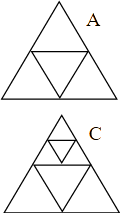
\includegraphics[width=0.95\columnwidth]{img/triangles1.png}
\end{minipage}
\hfill
\begin{minipage}{0.62\linewidth}\setlength{\parindent}{1.5em}
\begin{prf}
    Попробуем сначала разрезать треугольник на небольшое количество треугольников (см. рис.) Заметим, что разбив любой из участвующих в разбиении треугольник на 4 так, как на рисунке $A$, мы увеличиваем количество треугольников разбиения на 3. Тем самым можно легко получить последовательность разбиений с шагом 3. Откуда возникает идея доказательства. Итак, будем доказывать утверждение индукцией по количеству треугольников разбиения.
    \par
    \textit{\underline{База}}. Для $n$ = 6, 7 и 8 - рисунки $B$, $C$ и $D$ соответственно.
    \textit{\underline{Переход}}. Пусть доказано для количества треугольников $n = k$. Докажем для $n = k + 3$. Действительно, если есть разбиение на $k$ треугольников, то разбив один из них так, как на рисунке $A$, получим искомое. Тем самым переход доказан и утверждение доказано. 
\end{prf}
\end{minipage}
\hfill
\begin{minipage}{0.15\linewidth}
    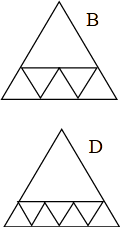
\includegraphics[width=0.95\columnwidth]{img/triangles2.png}
\end{minipage}
\end{figure}}

\begin{thm}
Докажите, что квадрат можно разрезать на любое количество квадратов, начиная с шести.
\end{thm}

\begin{thm}
Покемон Миша умеет рвать любой лист бумаги на 4 части, а покемон Гриша - на 6 частей. Докажите, что они смогут разобрать лист бумаги на любое количество кусков, начиная с девяти.
\end{thm}

\par

До сих пор мы говорили об индукции ''вверх'', т.е. когда мы поднимались от меньших значениях $n$ к большим. Заметим, что принципиальных различий в самом построении доказательства нет. Изменится база (теперь это будет не наименьшее возможное значение $n$, а наибольшее из возможных), и индукционный
переход будет осуществляться не от $k$ к $k + 1$, а от $k$ к $k - 1$.

\begin{ex}
Запишите, как выглядит схема доказательства для индукции в отрицательном направлении.
\end{ex}

\newpage

\section{Индукция в геометрии.}

{\setlength{\intextsep}{2pt}
\begin{figure}[h]
\begin{minipage}{0.3\linewidth}
    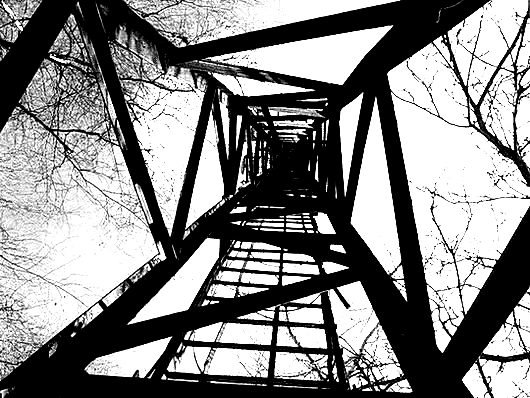
\includegraphics[width=0.95\columnwidth]{img/ladder.png}
\end{minipage}
\begin{minipage}{0.69\linewidth}\setlength{\parindent}{1.5em}
Применение индукция в геометрии является одним из наиболее сложных. Зачастую просто неясно, по какому параметру её следует вести. Кроме того, при доказательстве приходится использовать геометрические факты, необходимость которых в исходной формулировке не ощущается. Выше была разобрана задача о сумме углов выпуклого многоугольника. Докажем с помощью индукции эту формулу для произвольного многоугольника.
\end{minipage}
\hfill
\end{figure}}

\begin{dfn}
Многоугольником назовём замкнутую ломаную на плоскости без самопересечений.
\end{dfn}

\fbox{\begin{minipage}{0.95\textwidth}
    \textbf{Важный геометрический факт}. В любом многоугольнике найдётся диагональ, целиком лежащая внутри этого многоугольника.
\end{minipage}} 

\begin{thm}
Докажите, что сумма углов любого $n$-угольника равна $180 ^{\circ} \times (n - 2)$.
\end{thm}

\begin{prf}
Утверждение задачи имеет смысл при всех натуральных $n \geq 3$, поэтому и базой индукции будет соответственно $n = 3$.
\par
\textit{\underline{База}}. Утверждение $A_3$ верно по теореме о сумме углов треугольника.
\par
\textit{\underline{Индукционное предположение}}. Пусть утверждение верно для всех многоугольников с количеством углов, не превосходящим $k$.
\par
\textit{\underline{Переход}}. Рассмотрим произвольный $(k + 1)$-угольник. Согласно ''важному геометрического факту'' найдётся диагональ, лежащая целиком внутри этого многоугольника. Это значит, что эта диагональ разбивает данный многоугольник на два, причём количество углов в каждом из них заведомо меньше $(k + 1)$ (поскольку диагональ отсекает как минимум треугольник). Пусть у одного полученного многоугольника количество углов $m$, тогда у второго $(k + 1) - m + 2 = k - m + 3$.\footnotemark По
индукционному предположению для обоих многоугольников верна формула для суммы углов. Но сумма
углов исходного многоугольника равна сумме углов двух полученных многоугольников. Поэтому искомая сумма равна $180 ^{\circ} \times (m - 2) + 180 ^{\circ} \times (k - m + 3 - 2) = 180 ^{\circ} \times (k - 1) = 180 ^{\circ} ((k + 1) - 2)$. А это требуемая
формула для $(k + 1)$-угольника, что и требовалось доказать.
Тем самым переход доказан и всё утверждение доказано.
\end{prf}\footnotetext{Заметим, что для произвольной диагонали это неверно. Для невыпуклого многоугольника диагональ может пересекать стороны этого многоугольника.}

\begin{thm}
Докажите, что всякий (не обязательно выпуклый) многоугольник можно разделить на треугольники непересекающимися диагоналями.
\end{thm}

\begin{thm} $^{**}$
Докажите, что выпуклый многоугольник можно разрезать непересекающимися диагоналями на остроугольные треугольники не более, чем одним способом.
\end{thm}

\begin{thm}
Докажите, что если $n$ точек не лежат на одной прямой, то среди прямых, их соединяющих, не менее $n$ различных.
\end{thm}

\begin{thm} $^n$
Несколько кругов одного радиуса положили на стол так, что никакие два не перекрываются. Докажите, что круги можно раскрасить в четыре цвета так, что любые два касающихся круга будут разного цвета.
\end{thm}

\begin{thm} $^*$
Дан остроугольный треугольник $A_0B_0C_0$. Пусть точки $A_1$, $B_1$, $C_1$ — центры квадратов, построенных на сторонах $B_0C_0$, $C_0A_0$, $A_0B_0$. С треугольником $A_1B_1C_1$ делаем то же самое. Получаем треугольник $A_2B_2C_2$ и т.д. Доказать, что $\Delta A_{n + 1}B_{n + 1}C_{n + 1}$ пересекает $\Delta A_nB_nC_n$ ровно в 6 точках.
\end{thm}

\begin{thm} $^*$
    Докажите, что в выпуклом $n$-угольнике нельзя выбрать больше $n$ диагоналей так, чтобы любые две из них имели общую точку.
\end{thm}

\begin{thm}
    Вершины выпуклого многоугольника раскрашены в три цвета так, что каждый цвет присутствует, и никакие две соседние вершины не окрашены в один цвет. Докажите, что многоугольник можно разбить диагоналями на треугольники так, чтобы у каждого треугольника вершины были трёх разных цветов.
\end{thm}

\newpage

\begin{thm} $^{**}$
    На окружности радиуса 1 отмечена точка $O$ и из неё циркулем делается засечка вправо радиусом l. Из полученной точки $O_1$ в ту же сторону тем же радиусом делается вторая засечка, и так делается 2011 раз. После этого окружность разрезается во всех 2011 засечках, и получается 2011 дуг. Сколько дуг различных длин может при этом получиться?
\end{thm}

\section{Очень известные задачи.}

{\setlength{\intextsep}{2pt}
\begin{figure}[h]
\begin{minipage}{0.3\linewidth}
    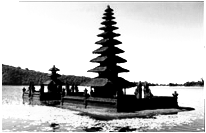
\includegraphics[scale=0.7]{img/sobor.png}
\end{minipage}
\begin{minipage}{0.69\linewidth}\setlength{\parindent}{1.5em}
\textit{
''В Великом храме города Бенарас, под собором, отмечающим середину мира, находится бронзовый диск, на котором укреплены 3 алмазных стержня, высотой в один локоть и толщиной с пчелу. При создании мира Бог Брама поместил на один из стержней 64 диска из чистого золота, причём так, что каждый меньший диск лежит на большем. Это и есть башня Брамы. День и ночь монахи в храме занимаются тем, что перекладывают диски в соответствии с наставлением Брамы так, чтобы меньший диск никогда не оказывался под большим. Как только все 64 диска будут переложены со стержня, на который Бог Брама сложил их при создании мира, на другой стержень, башня вместе с храмом обратятся в пыль и под громовые раскаты погибнет мир.''}
\par
\hspace*{0pt}\hfill \textit{Старинная легенда.}
\end{minipage}
\hfill
\end{figure}}

Традиционно применение индукции рассказывают, иллюстрируя очень известными примерами. Это так называемая классика жанра. Любой мало-мальски уважающий себя математик с такими примерами знаком. Часть таких классических задач были уже приведены выше (в частности задача \ref{6.0 thm1}). В этой же главе хочется привести решение ещё двух классических задач, без которых не обходится практически ни одно изложение метода индукции. В первую очередь это задача про головоломку ''Ханойская башня''.
{\setlength{\intextsep}{2pt}
\begin{figure}[h]
\begin{minipage}{0.69\linewidth}\setlength{\parindent}{1.5em}
Эта головоломка (иногда еще её называют ''Башня Брамы'' или ''Конец света'') придумана в 1883 году французским математиком Эдуардом Люка.\footnotemark На её создание его вдохновила старая легенда о
башне Брамы.
\par
\textbf{\textit{Игра ''Ханойская башня''}}. Имеется пирамида из $n$ колец, надетых на стержень, и два пустых стержня той же высоты. Диаметры колец убывают от основания пирамиды к её вершине (т.е. у основания находится самое большое кольцо, наверху - самое маленькое). Разрешается перекладывать верхнее кольцо с одного стержня на другой, но при этом запрещается класть большее кольцо на меньшее. Требуется переложить все кольца с одного стержня на другой.
\end{minipage}
\hfill
\begin{minipage}{0.25\linewidth}
    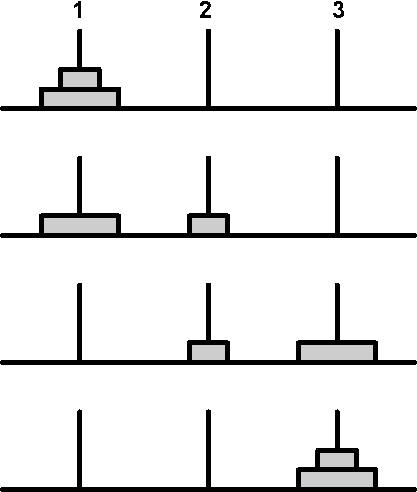
\includegraphics[width=0.95\columnwidth]{img/sobor_2.png}
\end{minipage}
\end{figure}}\footnotetext{Франсуа Эдуард Анатоль Люка (1842-1891) - французский математик, профессор. Работал в лицее Лунле-Гран в Париже. Важнейшие работы Люка относятся к теории чисел и неопределённому анализу. Считал, что с помощью машин или каких-либо приспособлений сложение удобнее производить в двоичной системе, чем в десятичной. Исследовал числе Мерсенна и обобщил понятия чисел Фибоначчи, получивших имя чисел Люка.}

\begin{thm}
Докажите, что можно переложить все кольца в игре Ханойская башня на один из пустых стержней, и что это можно сделать за $2n - 1$ перекладываний.
\end{thm}

\begin{prf}
Будем доказывать требуемое утверждение индукцией по количеству колец.
\par
\textit{\underline{База}}.
n = 1. Очевидно, что одно кольцо можно переложить за одно перекладывание, и что $2^1 - 1 = 1$.
\par
\textbf{\textit{Замечание.}} Несмотря на то, что совершенно верно в качестве базы рассматривать значение $n$, равное 1, чтобы показать, как происходят перекладывания, разберём случай для $n$ = 2.
\par
На рисунке изображена пирамидка с двумя кольцами и два пустых стержня. Стержни занумерованы числами от 1 до 3. На последующих рисунках изображено, как следует осуществлять перекладывания, чтобы переместить пирамидку с первого стержня на третий:
\par
\begin{center}
    $1 \rightarrow 2; 1 \rightarrow 3; 2 \rightarrow 3$.
\end{center}
\par
\textit{\underline{Предположение}}. Пусть утверждение верно для пирамидки с количеством колец $n = k$, т.е. мы можем переместить пирамидку из $k$ колец на другой стержень за $2^k - 1$
перекладываний. 
\par
\textit{\underline{Переход}}. Пусть теперь есть пирамидка из $n = k + 1$ колец. Будем считать, что самое нижнее - самое большое кольцо - неподвижно. Тогда оставшиеся $k$ колец можно переложить на другой стержень, не нарушая правила игры за $2^k - 1$ перекладываний. Заметим, что поскольку оставшееся кольцо самое большое, то на него можно класть любое из перекладываемых колец.
\end{prf}
\par
\begin{figure}[h]
\begin{minipage}{0.25\linewidth}
    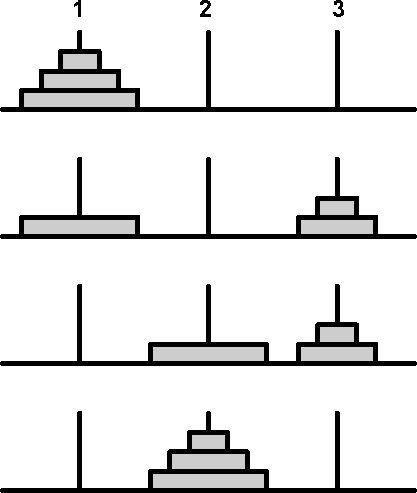
\includegraphics[width=0.95\columnwidth]{img/sobor_3.png}
\end{minipage}
\hfill
\begin{minipage}{0.69\linewidth}\setlength{\parindent}{1.5em}
Переложив пирамидку из $k$ колец, переложим $(k + 1)$-е кольцо на свободный стержень. Теперь переложим за $2^k - 1$ перекладываний пирамидку обратно на это кольцо. Всего получилось $2^k - 1 + 2^k - 1 + 1 = 2 \times 2^k - 1 = 2^{k + 1} - 1$ перекладываний, что и требовалось доказать.
\par
Заметим, что число перемещений дисков, которые должны совершить монахи в легенде, равно $2^{64}$ - 1 или 18 446 744 073 709 551 615. Если бы монахи, работая день и ночь, делали каждую секунду одно перемещение диска, их работа продолжалась бы 580 миллиардов лет.
\par
Заканчивая обсуждать эту задачу, остается только проиллюстрировать
переход от двух колец к трем (см.рис.)
\end{minipage}
\end{figure}
\begin{figure}[h]
\begin{minipage}{0.79\linewidth}\setlength{\parindent}{1.5em}
\begin{thm}
Плоскость поделена на области несколькими прямыми. Докажите, что эти области можно раскрасить в два цвета так, чтобы любые две соседние области были окрашены в разные цвета. (Соседними называются области, имеющие общий участок границы.)
\end{thm}
\par
\textbf{\textit{Замечание.}} Плоскость, поделённую на области какими-то линиями и раскрашенную в несколько цветов так, что точки одной области окрашены в один цвет, называют картой. Прежде всего, заметим, что не каждую карту можно раскрасить так, как требуется в условии задачи. Например, карту на рисунке требуемым образом раскрасить нельзя.
\end{minipage}
\hfill
\begin{minipage}{0.15\linewidth}
    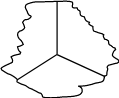
\includegraphics[width=0.95\columnwidth]{img/karta.png}
\end{minipage}
\end{figure}

\par

\begin{prf}
Будем доказывать требуемое утверждение индукцией по количеству прямых.
\begin{figure}[h]
\begin{minipage}{0.25\linewidth}
    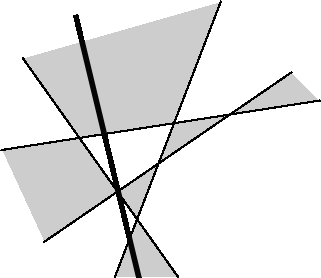
\includegraphics[width=0.95\columnwidth]{img/figura 6.0 1.png}
\end{minipage}
\hfill
\begin{minipage}{0.69\linewidth}\setlength{\parindent}{1.5em}
\textit{\underline{База}}. $n = 1$. Очевидно, что если прямая одна, то она делит всю плоскость на две полуплоскости и карту раскрасить можно: одну полуплоскость покрасим в белый цвет, а вторую - в чёрный.
\par
\textit{\underline{Предположение}}. Пусть утверждение верно для
$n = k$ прямых, т.е. мы можем раскрасить требуемым образом любую карту, образованную пересечением $k$ прямых.
\par
\textit{\underline{Переход}}. Рассмотрим карту из $n = k + 1$
прямых. Выберем какую-нибудь прямую и выкинем её из рассмотрения.
\end{minipage}
\end{figure}
\begin{figure}[H]
\begin{minipage}{0.25\linewidth}
    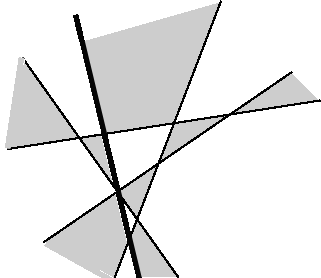
\includegraphics[width=0.95\columnwidth]{img/figura 6.0 2.png}
\end{minipage}
\hfill
\begin{minipage}{0.69\linewidth}\setlength{\parindent}{1.5em}
Тогда оставшиеся $k$ прямых образую карту, которую мы можем раскрасить. Сделаем это и вернем $(k + 1)$-ю прямую на место. Эта прямая делит всю плоскость на две полуплоскости. Чтобы построить раскраску для новой карты, в одной из плоскостей оставим раскраску областей такой, какая она есть, а в другой поменяем на противоположную, т.е. белые области перекрасим в чёрные, а чёрные - в белые. Почему новая раскраска будет удовлетворять условию? В каждой из полуплоскостей как граничили области разных цветов так и граничат. Новые границы могли появиться только за счет новой прямой. Если эта прямая делит какую-либо область на две части, то теперь эти части разных цветов, поскольку они находятся в разных полуплоскостях, а одну полуплоскость мы перекрашивали, а другую оставили без изменения.
\end{minipage}
\end{figure} 
\par
Тем самым переход доказан и все утверждение доказано. \end{prf}

\newpage

\begin{center}
    \textit{\textbf{Лирическое отступление.}}
\end{center}

\section*{Полная и неполная индукция.}

Говоря об индукции вообще, различают \textit{полную} и \textit{неполную} индукцию. Применяя полную индукцию, мы лишь тогда считаем себя вправе объявить об истинности универсальной формулировки, когда убедились в её истинности для каждого без исключения значения $n$. Метод неполной индукции состоит в переходе к универсальной формулировке после проверки истинности частных формулировок для отдельных, но не всех
значений $n$.

\begin{figure}[H]
\begin{minipage}{0.69\linewidth}\setlength{\parindent}{1.5em}
В повседневной жизни мы постоянно пользуемся методом неполной
индукции. Так, желая купить на рынке солёных огурцов, пробуем кусочек одного огурца (который протягивает нам продавец). Если он нравится, покупаем, например, 1 кг, рассудив так: "Если один огурец хороший, то и все хорошие". Это и есть метод неполной индукции в действии. Однако, не исключено, что все купленные огурцы окажутся плохими, кроме того одного, который мы попробовали. Другой пример. Магазин закупает партию яблок, и товаровед проверяет не одно яблоко, а по нескольку плодов из каждого ящика. 
\end{minipage}
\hfill
\begin{minipage}{0.3\linewidth}
    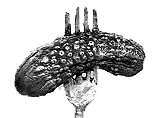
\includegraphics[width=0.95\columnwidth]{img/ogurec.png}
\end{minipage}
\end{figure} 
\par
Если выбранные яблоки спелые, то магазин примет решение ''все яблоки спелые'', т.е. также воспользуется методом неполной индукции, и закупит все ящики. Даже универсальные законы природы формулируются на основе отдельных наблюдений. А потому и наши повседневные решения (скажем, о качестве огурцов), и научные выводы (например, о законах природы), если они высказаны в виде универсальных формулировок, верны не абсолютно, а в лучшем случае лишь с высокой степенью правдоподобия.
\par
Иное дело математика. Метод неполной индукции, используемый в естественных науках, в математике не имеет права на существование. Нередко случается, что частная формулировка $A_n$ верна для отдельных значений $n$, и вместе с тем не удается найти таких значений, для которых она неверна. Тогда есть основание предположить, что универсальная формулировка истинна, - но только предположить, поскольку то, что не удалось найти сегодня, будет, возможно, открыто завтра. Вот ещё примеры (помимо примера
Эйлера, разобранного выше), говорящие о том, что метод неполной индукции в математике не работает.

\par

\textbf{\textit{Числа Ферма.}} Знаменитый математик XVII в. Пьер Ферма изучал числа вида $2^{2^n} + 1$. Их так и назвали - числа Ферма. Учёный полагал, что все эти числа простые. И у него на то, казалось бы, имелись основания: действительно, числа такого вида являются простыми при $n = 0, 1, 2, 3, 4$. Однако в XVIII в. Леонард Эйлер обнаружил, что при $n = 5$ это число равно произведению двух простых чисел $641$ и $6700417$. Более того, неизвестно, существуют ли простые числа Ферма помимо пяти вышеуказанных.

\par

\textbf{\textit{Части внутри окружности.}} На окружности взяли $n$ точек и соединили их всевозможными отрезками. Оказалось, что никакие три из этих отрезков не пересекаются в одной точке. На сколько частей они делят круг? При $n$ = 1, 2, 3, 4, 5 получаем соответственно 1, 2, 4, 8, 16 частей и напрашивается вывод, что
при любом $n$ количество частей равно $2^{n-1}$. А на самом деле их будет $$\dfrac{\dfrac{n(n - 1)(n - 2)(n - 3)}{24 + n(n - 1)}}{2+1}$$

\par

\textbf{\textit{Двучлен $x^n - 1$.}} Если разлагать двучлен $x^{n - 1}$ на множители при различных значениях $n$, то окажется, что у каждого из многочленов - сомножителей коэффициенты равны $\pm$ 1. Например, $x^6 - 1 = (x - 1)(x + 1)(x^2 + x + 1)(x^2 - x + 1)$. Гипотезу о том, что это справедливо для любого $n$ доказать, однако, почему-то не удавалось. А в 1941 г. выяснилось, что указанная особенность разложения двучлена $x^n - 1$ на множители существует при всех $n$ до 104 включительно, а в случае $n = 105$ появляется многочлен, отдельные коэффициенты которого равны -2.

\newpage

\textbf{\textit{Квадрат вида 991$\boldsymbol{n^2}$ + 1.}} Ещё один весьма убедительный пример. Подставляя в выражение $991n^2 + 1$ вместо $n$ последовательно целые числа 1, 2, 3, ... , мы никогда не получим числа, являющегося полным квадратом, сколько бы дней или даже лет мы ни посвятили этим вычислениям. Однако, если мы сделаем отсюда вывод о том, что все числа такого вида не являются квадратами, то мы ошибёмся. На самом деле, среди чисел вида $991n^2 + 1$ имеются квадраты, только наименьшее значение $n$, при котором число $991n^2 + 1$ есть полный квадрат, очень велико. Вот это число: $n$ = 12 055 735 790 331 359 447 442 538 767.

\section*{Парадокс кучи.}
Встретились два приятеля, стали разговаривать. Вдруг взгляд одного из них упал на кучу песка.

\par

\begin{figure}[H]
\begin{minipage}{0.64\linewidth}\setlength{\parindent}{1.5em}
- Видишь кучу песка? - спросил он. - А на самом деле её нет.
\par
- Почему? - удивился его приятель.
\par
- Очень просто, - ответил тот. - Давай рассудим: одна песчинка, очевидно, не образует кучи песка. Если $n$ песчинок не могут образовать кучи песка, то и после прибавления еще одной песчинки они по-прежнему не могут образовать кучи. Следовательно, никакое число песчинок не образует кучи, т.е. кучи песка нет.
\par
Мы только что описали известный \textit{парадокс кучи}.
\end{minipage}
\hfill
\begin{minipage}{0.35\linewidth}
    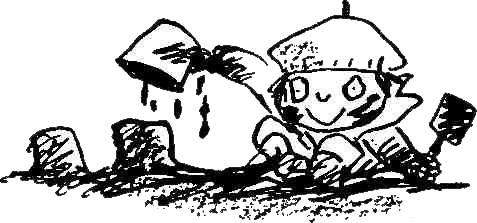
\includegraphics[width=0.95\columnwidth]{img/kucha.png}
\end{minipage}
\end{figure} 

\par

\begin{figure}[H]
\begin{minipage}{0.35\linewidth}
    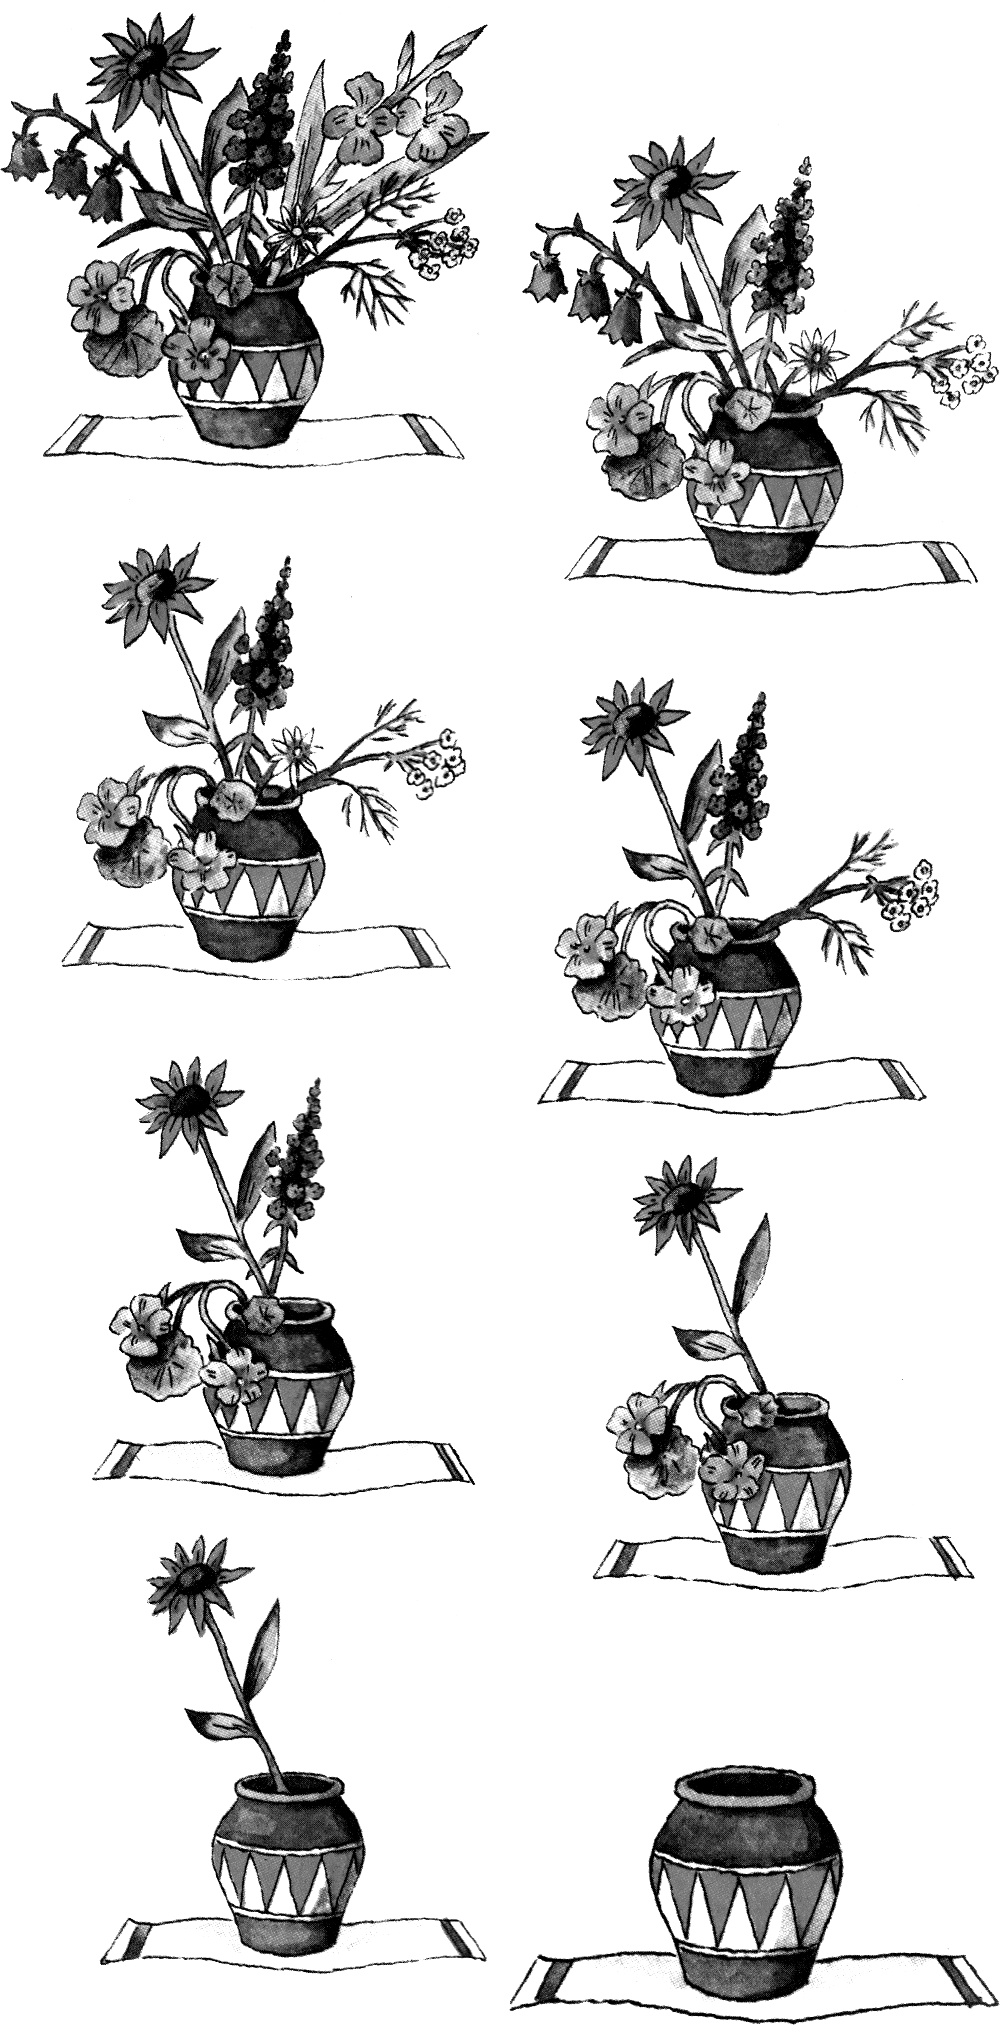
\includegraphics[width=0.95\columnwidth]{img/gorshok.png}
\end{minipage}
\hfill
\begin{minipage}{0.64\linewidth}\setlength{\parindent}{1.5em}
К этому парадоксу можно сделать следующий комментарий: метод полной математической индукции нельзя применять, как
показывает парадокс, к объёмно неопределённым понятиям,
каковым является понятие ''куча песка''. На рисунке слева
приведена иллюстрация к парадоксу букета.
\par
\begin{ex}
    Сформулируйте парадокс букета и объясните,
почему в данном случае не работает метод математической
индукции.
\end{ex}
Наконец-то мы подобрались к концу этого листка. Долго-долго мы шли от простейших примеров к достаточно сложным доказательствам. Теперь этот метод будет преследовать вас всюду. Это мощнейший инструмент математики, используйте его с умом. В заключение остаётся только добавить, что мы рассмотрели далеко не все схемы индукции. Но, зная основные приемы, вы легко сможете обосновать остальные. Заметим только, что бывает \textit{двойная индукция} (по двум переменным) или \textit{ветвящаяся индукция}, когда сначала утверждение доказывается не для всех $n$, а только для некоторых, например, для степеней двойки, а потом с помощью индукции в отрицательном направлении уже для остальных значений $n$. Кроме того, шаг индукции может быть не обязательно целым. А также бывает не только доказательство по индукции, но и определения по индукции. Например, когда члены некоторой последовательности, кроме нескольких первых, задаются индуктивно, т.е. через предыдущие. Так заданные последовательности называют \textit{рекуррентными} или \textit{возвратными}. Одной из наиболее известных рекуррентных последовательностей является ряд \textit{чисел Фибоначчи}: $Ф_1 = 1; Ф_2 = 1; Ф_n = Ф_{n - 1} + Ф_{n - 2}$. Числам Фибоначчи будет посвящен один из последующих листков.
\end{minipage}
\end{figure}

% \newpage

% \section*{УФФ!}



\section*{Для тех, кому показалось мало и не хочется расставаться с индукцией. \smiley}

\begin{thm}
    На химической конференции присутствовало $k$ учёных химиков и алхимиков, причём химиков было больше, чем алхимиков. Известно, что на любой вопрос химики всегда отвечают правду, а алхимики иногда говорят правду, а иногда лгут. Оказавшийся на конференции математик про каждого учёного хочет установить, химик тот или алхимик. Для этого он любому учёному может задать вопрос: ''Кем является такой-то: химиком или алхимиком?''. (В частности, может спросить, кем является сам этот учёный)

\par

Доказать, что математик может установить это за: 
\par
а) $4k$ вопросов;
\par 
б) $2k - 2$ вопросов.
\end{thm}

\begin{prf}
    Приводимое решение даёт возможность выяснить, кто - химик, а кто - алхимик, даже за меньшее, чем $2k - 2$, число вопросов, а именно за $q = 3m$ вопросов, если $k = 2m + 1$ - число нечётное, и за $3m - 2$ вопросов, если $k = 2m$ - число чётное. Вначале мы рассмотрим нечётные $k$. Искомый способ определим индукцией по $m$. 
    \par
    \textit{\underline{База}}. Если на конференции присутствовал $k = 1$ учёный $(m = 0)$, то он, очевидно, химик, поскольку химиков должно быть больше; никаких вопросов в этом случае задавать не надо: $q = 0 = 3 \times 0$. 
    \par
    \textit{\underline{Индукционное предположение}}. Предположим теперь, что для всех нечётных чисел, меньших данного числа $k = 2m + 1$, мы уже имеем способ, позволяющий решить задачу в требуемое число вопросов.
    \par
    \textit{\underline{Переход}}. Укажем такой способ для числа $k = 2m + 1$. Перенумеруем для удобства всех участников конференции произвольным образом и начнём спрашивать второго, третьего и т.д. учёных, кто есть первый учёный. Этот опрос мы прекратим, как только произойдёт одно из двух событий:
    \par
    \textbf{Событие A}. Среди опрошенных учёных большинство высказалось за то, что первый учёный — алхимик. 
    \par
    \textbf{Событие B}. Число учёных, утверждающих, что первый учёный - химик, равно $m$. Ясно, что если произошло \textbf{событие A}, и к этому моменту $t$ учёных утверждали, что первый учёный - химик, и $f$ - что он алхимик, то $f = t + 1$. (Действительно, $f > t$, а если предположить, что $f \geq t + 2$, то \textbf{событие A} должно произойти хотя бы на один вопрос раньше.) Ясно, кроме того, что при этом опросе было задано $q_1 = f + t = 2f - 1$ вопросов. (Частным случаем \textbf{события A} является ситуация, когда уже второй учёный сказал, что первый является алхимиком - здесь $t = 0, f = 1$.) Если же произошло \textbf{событие B} и при этом $f$ учёных утверждали, что первый учёный - алхимик, то общее число заданных вопросов равно $q_1 = m + f$.
    \par 
    Нетрудно видеть, что опрос прервётся до того, как будут опрошены все учёные, присутствующие на конференции. В самом деле, предположим противное. Значит, перед опросом последнего учёного не произошло ни одно из \textbf{событий A, B}. Пусть в этот момент среди опрошенных учёных $t$ человек высказались 6 за то, что первый учёный - химик и $f$ - за то, что он алхимик. Поскольку не произошло \textbf{события A}, $f \leq t$. Поскольку не произошло \textbf{события В}, $t \leq m - 1$. Поэтому общее число опрошенных $f + t \leq 2(m - 1)$. Добавив к ним первого и последнего учёных, мы получаем, что общее число участников конференции не превосходит $2m$, тогда как их $2m + 1$. Полученное противоречие доказывает, что одно из \textbf{событий} - \textbf{A} или \textbf{B} - произойдёт до того, как будет опрошен последний учёный.
    \par
    Пусть произошло \textbf{событие A}. Тогда мы утверждаем, что в группе учёных, состоящей из первого учёного и всех опрошенных учёных, число алхимиков не меньше числа химиков. Действительно, если первый учёный - химик, то те $f$ учёных, которые утверждали, что он алхимик, - сами алхимики. Поскольку общее число учёных в рассматриваемой группе есть $1 + t + f = 2f$, число алхимиков в группе в этом случае не меньше числа химиков. Если же первый учёный - алхимик, то алхимиками являются и те $t$ учёных, которые утверждали, что он химик. Поэтому и в этом случае число алхимиков не меньше $1 + t = f$, т.е. не меньше половины. Далее, поскольку общее число химиков превосходит по условию задачи общее число алхимиков, в оставшейся группе из $k - 2f = 2(m - f ) + 1$ учёных число химиков также должно превосходить число алхимиков. Число $k - 2f$, очевидно, меньше $k$, поэтому по \textit{\underline{предположению индукции}} существует способ, позволяющий за $q_2 = 3(m - f )$ вопросов выяснить, кто в оставшейся группе учёных есть химик и кто - алхимик. Выберем теперь из этой группы произвольного химика (такой, очевидно, найдётся) и спросим его (на это уйдёт $q_3 = 1$ вопрос), кто есть первый учёный. Если он алхимик, то те $t$ учёных, которые утверждали, что он химик, - алхимики. Поэтому нам остаётся лишь выяснить у выбранного нами химика, ''кто есть кто'' среди тех $f$ учёных, которые утверждали, что первый учёный - алхимик (на это уйдёт ещё $q_4 = f$ вопросов). В результате мы восстановим полную картину разбиения участников конференции на химиков и алхимиков и истратим на это $q = q_1 + q_2 + q_3 + q_4 = 2f - 1 + 3(m - f) + 1 + f = 3m$ вопросов, что и требовалось.
    \par
    Если же первый учёный оказался химиком, то те $f$ учёных, которые утверждали, что он алхимик, сами являются алхимиками. Поэтому нам остаётся выяснить у выбранного нами химика лишь ''кто есть кто'' в группе из $t$ учёных, утверждавших, что первый учёный - химик. На это мы затратим $q_4 = t$ вопросов. Общее число вопросов $q = q_1 + q_2 + q_3 + q_4 = 2f - 1 + 3(m - f ) + 1 + t = 3m - 1$ в этом случае даже меньше того числа вопросов, которое мы вправе использовать. Тем самым случай, когда произошло \textbf{событие A}, полностью разобран.
    \par
    Рассмотрим теперь тот случай, когда произошло \textbf{событие B}. Мы утверждаем, что в этом случае первый учёный - химик. В самом деле, если бы он был алхимиком, то и те $m$ учёных, которые утверждали, что он химик, тоже были алхимиками и общее число алхимиков было бы не меньше $m + 1$, т.е. больше половины, а это противоречит условию задачи. Итак, первый учёный - химик, а те $f$ учёных, которые утверждали, что он алхимик, сами - алхимики. Выясним теперь у первого учёного ''кто есть кто'' среди тех $m$ учёных, которые утверждали, что он химик (на это уйдёт $q_2 = m$ вопросов), и ''кто есть кто'' среди остальных учёных, не участвовавших в опросе (на это уйдёт ещё $q_3 = k - (1 + m + f) = 2m + 1 - 1 - m - f = m - f$ вопросов). Таким образом, мы полностью выясним ''кто есть кто'' на конференции и затратим на это $q = q_1 + q_2 + q_3 = m + f + m + m - f = 3m$ вопросов. Тем самым оба случая - и когда происходит \textbf{событие A}, и когда происходит \textbf{событие B} - рассмотрены, и поэтому для нечётного числа участников задача полностью решена. Пусть теперь $k = 2m$ - чётное число. Удалим одного участника. По доказанному, за $3m-1$ вопрос мы узнаем ''кто есть кто''. С помощью ещё одного вопроса, заданного химику, мы узнаем, кем является последний участник.
\end{prf}

\begin{ex}
    Прочитайте решение предыдущей задачи не менее трёх раз.
\end{ex}

\begin{ex}
    Разберитесь в решении предыдущей задачи.
\end{ex}

\begin{thm}
    Докажите пункт а) предыдущей задачи более простым способом...
\end{thm}

\par

\textbf{\textit{Фокусы по индукции.}} Вырежьте из картона 999 одинаковых карточек. На 111 карточках напишите 1, на 111 карточках - 2, и т.д., на последних 111 карточках напишите 9. Переверните все карточки цифрой вниз и тщательно перемешайте. Затем возьмите совершенно произвольно $n$ карточек, где $n$ - любое целое число от 1 до 100, и положите их на стол цифрой вверх. Тогда цифры, написанные на всех $n$ выбранных карточках, обязательно окажутся одинаковыми! Сколько бы раз ни повторять этот фокус и какое бы $n$ ни выбирать $(1 \leq n \leq 100)$, результат неизменно будет один: на всех $n$ карточках будет одна и та же цифра! Каждый может на досуге проверить сказанное экспериментально.

\begin{thm} $^*$
    На плоскости даны $2n + 1$ точек. Постройте ($2n + 1$)-угольник, для которого эти точки являются серединами сторон.
\end{thm}

\begin{thm} $^*$
    Докажите, что шахматную доску $2007 \times 2007$ можно обойти ходом шахматного коня, побывав на каждом поле ровно один раз.
\end{thm}

\begin{thm} $^*$
    В некотором государстве каждые два города соединены дорогой. На каждой дороге разрешено движение только в одну сторону. Докажите, что найдётся город, выехав из которого можно объехать все государство, побывав в каждом городе ровно один раз.
\end{thm}

\begin{thm} $^*$
    Двум гениальным математикам сообщили по натуральному числу и сказали, что эти числа отличаются на единицу. После этого они по очереди задают друг другу один и тот же вопрос: ''Знаешь ли ты моё число?''. Докажите, что рано или поздно один из них ответит положительно.
\end{thm}

\begin{thm} $^*$
    На круглом барабане 64 сектора. Докажите, что в каждый сектор можно записать шестизначное число из цифр 1 и 2 так, чтобы все числа были различными и любые два соседних различались ровно в одном разряде.
\end{thm}

\begin{thm} $^*$
    Из чисел от 1 до $2n$ выбрано $n + 1$ число. Докажите, что среди выбранных чисел найдутся два, одно из которых делится на другое.
\end{thm}